\documentclass[10pt]{beamer}

% %%% Style %%%
\mode<presentation>
{
  \usetheme{Berlin}
  \setbeamertemplate{blocks}[rounded]
  \setbeamercolor{block title}{bg=gray}
  \setbeamercovered{transparent}
}

% %%% Packages %%%
% Babel and fonts
\usepackage[english]{babel}
\usepackage[utf8]{inputenc}

% Graphics and images
\usepackage{xcolor}
\usepackage{graphicx}
\DeclareGraphicsExtensions{.pdf,.png,.jpg, .eps}
\usepackage{relsize}
\usepackage{colortbl}


% Math notation and symbols
\usepackage{mathrsfs}
\usepackage{amsthm}
\usepackage{bbold}
\usepackage{amsfonts}
\usepackage{amsmath}
\usepackage{amssymb}
% \usepackage{algorithm}
\usepackage{algpseudocode}
\usepackage{listings}

% \DeclareMathOperator*{\len}{\text{length of }}
% Backup slides
\usepackage{appendixnumberbeamer}

% Tables, Colums and the like
\usepackage{longtable}
\usepackage{listings}

% Hyperref
\usepackage{hyperref} 

% Boxes
\usepackage{fancybox}
\usepackage{lmodern}
\usepackage{tikz}
\usepackage{tcolorbox}
\usepackage{mdframed}	

\usepackage{hyperref}
\usepackage{listings}
\usepackage{setspace}
\usepackage{subfiles}
\usepackage{alltt}
\usepackage{mathtools}
\usepackage{fancyvrb}
\usepackage{url}

\usepackage{tikz}
\usetikzlibrary{shapes,arrows,positioning,calc}

\usepackage{xparse}
\usepackage{ifthen}
\usepackage{twoopt}

% Custom packages (needs absolute path from root document
%  Usage: \usepackage{appendixnumberbeamer}
%  Custom title page

\makeatletter

\setbeamertemplate{footline}
{
  \leavevmode%
  \hbox{%
  \begin{beamercolorbox}[wd=0.25\paperwidth,ht=2.25ex,dp=1ex,center]{author in head/foot}%
    \usebeamerfont{author in head/foot}\insertshortauthor
  \end{beamercolorbox}%
  \begin{beamercolorbox}[wd=0.50\paperwidth,ht=2.25ex,dp=1ex,center]{title in head/foot}%
    \usebeamerfont{title in head/foot}\inserttitle
  \end{beamercolorbox}%
  \begin{beamercolorbox}[wd=0.25\paperwidth,ht=2.25ex,dp=1ex,right]{date in head/foot}%
    \insertframenumber{} / \inserttotalframenumber\hspace*{2ex} 
  \end{beamercolorbox}}%
  \vskip0pt%
}
\makeatother

\makeatletter
\setbeamertemplate{headline}
{
  \leavevmode%
  \hbox{%
  \begin{beamercolorbox}[wd=\paperwidth,ht=2.25ex,dp=1ex,center]{title in head/foot}%
  \end{beamercolorbox}%
  }%
  \vskip0pt%
}
\makeatother

\defbeamertemplate*{title page}{customized}[1][]
{
  \begin{center}
    \begin{variableblock}{}{}{bg=blue}
      \begin{center}
	\usebeamerfont{title}\inserttitle\par
      \end{center}
    \end{variableblock}
  \end{center}

  \begin{center}
    \begin{minipage}{1.0\textwidth}
      \begin{center}
	\insertauthor

	\begin{scriptsize}
	  \insertdate
	\end{scriptsize}

      \end{center}
    \end{minipage}
  \end{center}
}

% vim:ft=plaintex:
%
%  Written and (C) by J�r�me Lelong <jerome.lelong@gmail.com>
%  2007 - 2012
% 
%  This program is free software; you can redistribute it and/or modify it
%  under the terms of the GNU General Public License as published by the
%  Free Software Foundation; either version 3 of the License, or (at your
%  option) any later version.
% 
%  This program is distributed in the hope that it will be useful, but
%  WITHOUT ANY WARRANTY; without even the implied warranty of
%  MERCHANTABILITY or FITNESS FOR A PARTICULAR PURPOSE.  See the GNU
%  General Public License for more details.
% 
%  You should have received a copy of the GNU General Public License along
%  with this program.  If not, see <http://www.gnu.org/licenses/>. 
% 
%  This small piece of code fixes the frame numbering in beamer when using
%  an appendix such  that the slides of the appendix are not counted in the
%  total framenumber of the main part of the document. The total
%  framenumber counter is reset to 0 and starts counting again when
%  entering the appendix.
% 
%  Usage: \usepackage{appendixnumberbeamer}
%  and declare the appendix as usual using the \appendix command.


\makeatletter


\let\appendixtotalframenumber\empty
\def\mainend{-1}
\let\appendixorig\appendix

% Redefine the \appendix command:
%   - it resets the framenumber counter 
%   - freezes the total framenumber for this first part of the document
\def\appendix{
  \edef\mainend{\theframenumber}
  \immediate\write\@auxout{\string\global\string\@namedef{mainendframenumber}{\mainend}}
  \appendixorig
  \def\inserttotalframenumber{\appendixtotalframenumber}%
  \setcounter{framenumber}{0}
}

% To be called at the end of document to fix the total framenumber in the
% main document and in the appendix.
\def\pageatend{
  \edef\appendixend{\theframenumber}
  \ifnum\mainend>0%
  \immediate\write\@auxout{\string\global\string\@namedef{appendixtotalframenumber}{\appendixend}}%
  \immediate\write\@auxout{\string\global\string\@namedef{inserttotalframenumber}{\mainend}}%
  \immediate\write\@auxout{\string\@writefile{nav}{\noexpand \headcommand {%
        \noexpand \def\noexpand \inserttotalframenumber{\mainend}}}}%
  \immediate\write\@auxout{\string\@writefile{nav}{\noexpand \headcommand {%
        \noexpand \def\noexpand \appendixtotalframenumber{\appendixend}}}}%
  \else
  \fi
}


\AtEndDocument{\pageatend}
\makeatother


% %%% Macros and custom commands %%%
\DeclareMathOperator*{\len}{\textbf{length of }}

\newcommand{\btVFill}{\vskip0pt plus 1filll}

\setbeamercolor{structure}{fg=cyan!90!black}

\newenvironment{variableblock}[3]{%
\setbeamercolor{block body}{#2}
\setbeamercolor{block title}{#3}
\begin{block}{#1}}{\end{block}}

\lstdefinestyle{JavaPlain}{ %
basicstyle=\scriptsize\ttfamily, % the size of the fonts 
numbers=left,                   % where to put the line-numbers
numberstyle=\tiny,      % the size of the fonts that are used for th
stepnumber=1,                   % the step between two line-numbers
numbersep=5pt,                  % how far the line-numbers are from the code
backgroundcolor=\color{white},  % choose the background color
showspaces=false,               % show spaces adding particular underscores
showstringspaces=false,         % underline spaces within strings
showtabs=false,                 % show tabs within strings adding 
frame=single,           % adds a frame around the code
tabsize=2,          % sets default tabsize to 2 spaces
captionpos=b,           % sets the caption-position to bottom
breaklines=true,        % sets automatic line breaking
breakatwhitespace=false,    % sets if automatic breaks should only happen
fancyvrb=true,
fvcmdparams=textbf 1 textit 1,
}

% Colors
\definecolor{ballblue}{rgb}{0.13, 0.67, 0.8}
\definecolor{brown(web)}{rgb}{0.65, 0.16, 0.16}
\definecolor{brown(traditional)}{rgb}{0.59, 0.29, 0.0}

\newcommand\Red[1]{\textcolor{red}{#1}}
\newcommand\Green[1]{\textcolor{green!50!black}{#1}}
\newcommand\LightGreen[1]{\textcolor{green!60!black}{#1}}
\newcommand\Blue[1]{\textcolor{blue!60!white}{#1}}
\newcommand\Violet[1]{\textcolor{violet}{#1}}
\newcommand\LightBlue[1]{\textcolor{ballblue}{#1}}
\newcommand\Grey[1]{\textcolor{gray}{#1}}
\newcommand\Gray[1]{\textcolor{gray}{#1}}
\newcommand\Brown[1]{\textcolor{brown(web)}{#1}}
\newcommand\LightBrown[1]{\textcolor{brown(traditional)}{#1}}

% Helpers
\newcommand\Jcomment[1]{\LightGreen{// #1}}
\newcommand\JcommentMulti[1]{\LightGreen{/* #1}}
\newcommand\String[1]{\textcolor{blue!80!blue}{#1}}
\newcommand\Word[1]{\textcolor{purple!90!red}{#1}}
\newcommand\bang{!}
\newcommand\pipe{\|}

% Prints
% \newcommand\Jprintf[2][]{\LightBlue{printf}(\String{#1}, #2)}
\newcommandtwoopt{\Jprintf}[2][-NoValue-][-NoValue-]{%
    \ifthenelse{\equal{#2}{-NoValue-}}{\LightBlue{printf}(\String{#1})}{\LightBlue{printf}(\String{#1}, #2)}%
}

\newcommand\Jprintln[1]{\LightBlue{println}(\String{#1})}
\newcommand\JprintLN{\LightBlue{println}}

% Control structures
% Shortcut for JavaFor:
% \JavaFor (\Blue!init| \Green!n <= Math.sqrt(numero);| \Violet!n++|)
\newcommand\JavaForColors[3]{\Blue{#1}; \Green{#2}; \Violet{#3}}

\newcommand\Jfor[1][-NoValue-]{%
  \ifthenelse{\equal{#1}{-NoValue-}}{\Word{for}}{\JavaForO[#1]}%
}

\newcommandtwoopt{\JavaForO}[3][-NoValue-][-NoValue-]{%
    \JavaForOptions{#1}{#2}{#3}%
}

\DeclareDocumentCommand\JavaForOptions{ ggg }{%
  \Word{for}\IfValueT{#1}{%
    (\JavaForColors{#1}{#2}{#3}) %
  }%
}

% Shortcut for JavaFor:
% \JavaFor (\Blue!init| \Green!n <= Math.sqrt(numero);| \Violet!n++|)
\newcommand\Jif[1][-NoValue-]{%
  \ifthenelse{\equal{#1}{-NoValue-}}{\Word{if}}{\Word{if} (\Green{#1})}%
}

% Other reserved words
\newcommand\Jstatic{\Word{static}}
\newcommand\Jpublic{\Word{public}}
\newcommand\Jprivate{\Word{private}}
\newcommand\Jdouble{\Word{double}}
\newcommand\Jfloat{\Word{float}}
\newcommand\Jint{\Word{int}}
\newcommand\Jvoid{\Word{void}}
\newcommand\Jreturn{\Word{return}}
\newcommand\Jclass{\Word{class}}
\newcommand\Jargs{\LightBrown{args}}

\newenvironment{JavaCodePlain}[1][]
  { \VerbatimEnvironment%
    \begin{Verbatim}[#1]}
  { \end{Verbatim}  } 

\algdef{SE}[DOWHILE]{Do}{DoWhile}{\algorithmicdo}[1]{\algorithmicwhile\ #1}%
\renewcommand{\algorithmicrequire}{\textbf{Input:}}
\renewcommand{\algorithmicensure}{\textbf{Output:}}

\title[Laboratorio di Informatica - Lezione 5]{Laboratorio di Informatica \\ Lezione 5}
\author[Cristian Consonni]{Cristian Consonni}
\date[28/10/2015]{11 novembre 2015}
\institute[UniTN]{Università degli Studi di Trento}

% %%% Put slides with section name at the begining of each section %%%
\AtBeginSection[]
{
  \begin{frame}<beamer>
    \frametitle{Outline for section \thesection}
    \tableofcontents[currentsection]
  \end{frame}
}
\setbeamertemplate{navigation symbols}{}

\begin{document}

%%%%%%%%%% TITLE %%%%%%%%%%
% Formerly part of title.tex
\begin{frame}
  \titlepage
\end{frame}

\begin{frame}{Outline}
  \tableofcontents
\end{frame}
%%%%%%%%%% END TITLE %%%%%%%%%%

\subsection[Informazioni generali]{Informazioni generali}

\begin{frame}{Chi sono}
  Cristian Consonni

  \begin{itemize}
    \item \textbf{DISI - Dipartimento di Ingegneria e Scienza dell'Informazione}
    \item \textbf{Pagina web} del laboratorio: \structure{\url{http://disi.unitn.it/~consonni/teaching}}
    \item \textbf{Email}: \structure{\url{cristian.consonni@unitn.it}}
    \item \textbf{Ufficio}: Povo 2 - Open Space 9
      \begin{itemize}
	\item Per domande: scrivetemi una mail
	\item Ricevimento: su appuntamento via mail
      \end{itemize}
  \end{itemize}
\end{frame}



\begin{frame}{Obiettivi del laboratorio}
  Obiettivi del laboratorio:
  \begin{itemize}
    \item Apprendere i fondamenti di un vero linguaggio di programmazione (Java)
    \item Svolgere il progetto
  \end{itemize}

  Obiettivi del laboratorio
  \begin{enumerate}
    \item Fare esperienza in laboratorio
    \item Raggiungere una buona manualità nell'uso degli strumenti standard
    \item Esercizi
  \end{enumerate}

\end{frame}

\pgfdeclareimage[width=0.6\paperwidth]{xkcd}{img/11th_grade.png}
\begin{frame}{Manualità (I)}
  \begin{center}
    \pgfuseimage{xkcd}
  \end{center}
  \url{https://xkcd.com/519/}
\end{frame}

\pgfdeclareimage[width=0.6\paperwidth]{abstrusegoose}{img/ars_longa_vita_brevis.png}
\begin{frame}{Manualità (II)}
  \textbf{How to Teach Yourself Programming:}\footnote{\url{http://abstrusegoose.com/249}}
  \begin{center}
    \pgfuseimage{abstrusegoose}
  \end{center}
  
\end{frame}

\begin{frame}{Slides}

  Info sulle slide:
  \begin{itemize}
    \item le slide del corso saranno rese disponibili sul sito;
    \item segnalate pure eventuali errori;
    \item cercherò di pubblicare le slide in anticipo rispetto alla lezione;
    \item queste slide sono prodotte con \LaTeX \; \texttt{Beamer} (\emph{usate} \LaTeX!);
  \end{itemize}

  Segnalazioni di materiale:
  \begin{itemize}
    \item Materiale da voi prodotto;
    \item Cose interessanti che trovate online;
    \item Possiamo valutare insieme se riutilizzarle;
  \end{itemize}
\end{frame}

\section{Introduzione alla Programmazione Orientata agli Oggetti (OOP)}
\begin{frame}{Programmazione Orientata agli Oggetti (I)}
  
  \begin{itemize}
   \item La Programmazione Orientata agli Oggetti (o \emph{Object Oriented Programming}, OOP, in inglese)
         è un paradigma di Programmazione basato sui concetti di \textbf{oggetto} e \textbf{classe}.
   \item In questa lezione introdurremo i concetti di base legati agli oggetti e li utilizzeremo
         come una \textbf{struttura dati}, ovvero una entità che permette di gestire un insieme di
         dati (detti \emph{attributi} o \emph{membri}).
  \end{itemize}

\end{frame}

\begin{frame}{Programmazione Orientata agli Oggetti (II)}
  
  Finora \textbf{\Red{ad eccezione delle \texttt{String}}} abbiamo usato delle variabili di uno dei
  tipi \textbf{primitivi} (o \emph{atomici}):
  \begin{itemize}
    \item \texttt{\Word{int}}
    \item \texttt{\Word{double}}
    \item \texttt{\Word{float}}
    \item \dots
  \end{itemize}
  

  utilizzando un tipo primitivo sappiamo che i dati verrano rappresentati in memeria in un 
  un modo predefinito:
  \begin{itemize}
   \item \texttt{\Word{int}} $\rightarrow$ 4 byte (32 bit) 
   \begin{itemize}
    \item min: $-2^{31}$;
    \item max: $2^{31} - 1$;
   \end{itemize}

   \item \texttt{\Word{double}} $\rightarrow$ 8 byte (64 bit)
   \begin{itemize}
    \item $max \equiv |min|$: $1.7976931348623157 \cdot 10^{308}$;
    \item $\varepsilon$: $4.9 \cdot 10^{-324}$;
   \end{itemize}
  \end{itemize}

\end{frame}

\begin{frame}[fragile]\frametitle{Programmazione Orientata agli Oggetti (III)}
  
  Immaginiamo di volere scrivere un programma che memorizza i dati (nome e cognome,
  luogo di nascita, età) di una persona.
  \begin{JavaCodePlain}[commandchars=\\!|]
  
  String nome1 = \String!"Alice Rossi"|;
  String luogo1 = \String!"Milano"|;
  \Jint eta1 = 19;
  
  String nome2 = \String!"Roberto Verdi"|;
  String cognome2 = \String!"Roma"|;
  \Jint  eta2 = 20;
  \dots

  \end{JavaCodePlain}
  
  Problemi di questo approccio:
  \begin{itemize}
   \item   È molto scomodo creare nuove istanze dell'entità (concettuale) ``Persona'';
   \item   È molto facile commettere errori;
  \end{itemize}

\end{frame}

\begin{frame}[fragile]\frametitle{Programmazione Orientata agli Oggetti (IV)}

  Una \textbf{oggetto}:
  \begin{itemize}
    \item è un'\emph{entità software} costituito da un insieme di stati e comportamenti che si riferiscono a uno stesso concetto; \\
          {\footnotesize (\emph{«An object is a software bundle of related state and behavior.»}) }
          {\scriptsize \LightBlue{\url{https://docs.oracle.com/javase/tutorial/java/concepts/}} }
    \item consiste in una regione di memoria allocata;

  \end{itemize}
\end{frame}

\begin{frame}[fragile]\frametitle{Programmazione Orientata agli Oggetti (V)}

  Una \textbf{classe}:
  \begin{itemize}
    \item è un prototipo a partire dalla quale gli oggetti vengono \textbf{creati} (o \textbf{istanziati}, 
	  o \textbf{instanziati});\\
          {\footnotesize (\emph{«A class is a blueprint or prototype from which objects are created.»}) }
          {\scriptsize \LightBlue{\url{https://docs.oracle.com/javase/tutorial/java/concepts/}} }
    \item è la specifica che descrive quali sono i possibili stati e comportamenti di un oggetto creati
          a partire da esso;
    \item è un insieme di variabili (anche dette \textbf{\emph{membri}} o \textbf{\emph{attributi}}) e di
         funzioni i metodi (dette \textbf{\emph{metodi}});
    \item è anche chiamata \emph{Abstract Data Type} (ADT).
  \end{itemize}
\end{frame}


\pgfdeclareimage[width=0.35\paperwidth]{people01}{img/people_jumping_01.png}
\pgfdeclareimage[width=0.35\paperwidth]{people02}{img/people_jumping_02.png}
\pgfdeclareimage[width=0.35\paperwidth]{people03}{img/people_jumping_03.png}

\begin{frame}[fragile]\frametitle{Programmazione Orientata agli Oggetti (VI)}


  \begin{columns}[T]
    \begin{column}[T]{7cm}
    Classe:
    \begin{JavaCodePlain}[commandchars=\\!|]
    
    \Jpublic \Jclass Persona {

      \Jprivate String nome;      
      \Jprivate String luogoNascita;
      \Jprivate \Jint eta;

    }

    \end{JavaCodePlain}
    \end{column}

    \begin{column}[T]{5cm}
    Oggetti:
    \begin{center}
      \pgfuseimage{people01}
    \end{center}
    \end{column}
  \end{columns}


  \begin{minipage}[b]{12cm}
  {\scriptsize Photo credit: CC-BY-SA Mark Sebastian @ Wikimedia Commons \url{http://bit.ly/1kip83N}}
  \end{minipage}
\end{frame}

\begin{frame}[fragile]\frametitle{Programmazione Orientata agli Oggetti (VI)}


  \begin{columns}[T]
    \begin{column}[T]{7cm}
    Classe:
    \begin{JavaCodePlain}[commandchars=\\!|]
    
    \Jpublic \Jclass Persona {

      \Jprivate String nome;      
      \Jprivate String luogoNascita;
      \Jprivate \Jint eta;

    }
    
    \dots
    
    Persona Alice;

    \end{JavaCodePlain}
    \end{column}

    \begin{column}[T]{5cm}
    Oggetti:
    \begin{center}
      \pgfuseimage{people02}
    \end{center}
    \end{column}
  \end{columns}

\end{frame}

\begin{frame}[fragile]\frametitle{Programmazione Orientata agli Oggetti (VI)}


  \begin{columns}[T]
    \begin{column}[T]{7cm}
    Classe:
    \begin{JavaCodePlain}[commandchars=\\!|]
    
    \Jpublic \Jclass Persona {

      \Jprivate String nome;      
      \Jprivate String luogoNascita;
      \Jprivate \Jint eta;

    }

    \dots
    
    Persona Alice;
    Persona John;

    \end{JavaCodePlain}
    \end{column}

    \begin{column}[T]{5cm}
    Oggetti:
    \begin{center}
      \pgfuseimage{people03}
    \end{center}
    \end{column}
  \end{columns}
  
\end{frame}

\begin{frame}[fragile]\frametitle{Programmazione Orientata agli Oggetti (VI)}


  \begin{columns}[T]
    \begin{column}[T]{7cm}
    Classe:
    \begin{JavaCodePlain}[commandchars=\\!|]
    
    \Jpublic \Jclass Persona {

      \Jprivate String nome;      
      \Jprivate String luogoNascita;
      \Jprivate \Jint eta;

    }

    \dots
    
    Persona Alice;
    Persona John;

    \end{JavaCodePlain}
    \end{column}

    \begin{column}[T]{5cm}
    Oggetti:
    \begin{center}
      \pgfuseimage{people03}
    \end{center}
    \end{column}
  \end{columns}

  \begin{alertblock}{Oggetti vs. Classi}
    Un oggetto è un'istanza di una classe
  \end{alertblock}
  
\end{frame}

\begin{frame}[fragile]\frametitle{Classi vs. Oggetti (I)}

  \begin{columns}
    \begin{column}{6cm}
      Classe:
      \begin{itemize}
	\item descrizione delle proprietà \emph{comuni} a una tipologia di variabili;
	\item \`e un ``concetto'';
	\item \`e una parte di un programma;
      \end{itemize}
      
%       \begin{enumerate}
%        \item Persona
%        \item Album
%        \item Canzoni
%       \end{enumerate}
    \end{column}

    \begin{column}{6cm}
      Oggetti:
      \begin{itemize}
	\item rappresentazioni delle proprietà di una singola istanza;
	\item Un ``fenomeno''/``manifestazione''.
	\item una parte dei dati nell'esecuzione di un programma.
      \end{itemize}
      
%       \begin{enumerate}
%        \item Hillary Clinton, Rafael Nadal, Lewis Hamilton;
%        \item Thriller, Back in Black, The Dark Side of the Moon
%        \item {\scriptsize Thriller, Beat it, Billie Jean, Hells Bells, Shoot to Thrill, Back in Black, \dots}
%       \end{enumerate}
    \end{column}
  \end{columns}

  ${}$
  \begin{columns}[T]
    \begin{column}[T]{6cm}
      \begin{enumerate}
       \item Persona
       \item Album
       \item Canzoni
      \end{enumerate}
    \end{column}

    \begin{column}[T]{6cm}    
      \begin{enumerate}
       \item Hillary Clinton, Rafael Nadal, Lewis Hamilton;
       \item Thriller, Back in Black, The Dark Side of the Moon
       \item {\small Thriller, Beat it, Billie Jean, Hells Bells, Shoot to Thrill, Back in Black, \dots}
      \end{enumerate}
    \end{column}
  \end{columns}

\end{frame}

\pgfdeclareimage[width=0.25\paperwidth]{people01}{img/muffins.jpg}
\begin{frame}[fragile]\frametitle{Classi vs. Oggetti (II)}

  \begin{itemize}
   \item Nella programmazione ad oggetti (OOP) si scrivono classi;
    \begin{itemize}
      \item il codice sorgente che scriviamo contiene delle \textbf{classi};
      \item una classe è ``statica'';
      \item ``Una'';
    \end{itemize}
   \end{itemize}

   \begin{itemize}
   \item Gli oggetti sono creati a partire dalle classi;
    \begin{itemize}
      \item una classe è come una ricetta di una torta, gli oggetti sono le torte prodotte
      a partire dalla ricetta.
      \item un oggetto è ``dinamico''
      \item ``Molti''
    \end{itemize}
  \end{itemize}

  ${}$
  \begin{columns}[T]
    \begin{column}[T]{4cm}
      Ricetta (Classe) \textbf{Muffin}:
      \begin{enumerate}
       \item 3 uova;
       \item 380 g di farina;
       \item \dots
      \end{enumerate}
    \end{column}

    \begin{column}[T]{7cm}    
     \pgfuseimage{people01}
    \end{column}
  \end{columns}
  ${}$
  {\scriptsize Photo credit: CC-BY Sara K @ Flickr \url{http://bit.ly/1kioQdd}}
\end{frame}

\section{Oggetti e Classi}

\begin{frame}[fragile]\frametitle{Classi: costruttore (I)}

  Una classe necessita di un \textbf{costruttore} per potere essere istanziata:
  
  \begin{JavaCodePlain}[commandchars=\\!|]
  \Jpublic \Jclass Persona {
    \Jcomment!attributi della classe -> variabili dell'oggetto|
    \Jprivate String nome;      
    \Jprivate String luogoNascita;
    \Jprivate \Jint eta;

    \Jcomment!Costruttore con parametri|
    \Jpublic Persona(String nome, String luogoNascita, \Jint eta) {
      \dots
    }

    \Jcomment!Costruttore senza parametri con valori di default|
    \Jpublic Persona() {
      \dots
    }    
  }
  \end{JavaCodePlain}

\end{frame}

\begin{frame}[fragile]\frametitle{Classi: costruttore (II)}

  Il \textbf{costruttore} è il \emph{metodo} che crea la classe:
  
  \begin{JavaCodePlain}[commandchars=\\!|]
  \Jpublic \Jclass Persona {
    \dots
    \Jcomment!Costruttore con parametri|
    \Jpublic Persona(String nome, String luogoNascita, \Jint eta) {
      \Jthis.nome = nome;
      \Jthis.luogoNascita = luogo;
      \Jthis.eta = eta;
    }

    \Jcomment!Costruttore senza parametri con valori di default|
    \Jpublic Persona() {
      \Jthis.nome = \String!"Anonimo"|;
      \Jthis.luogoNascita = \String!"Sconosciuto"|;
      \Jthis.eta = -1;
    }
  }
  \end{JavaCodePlain}

\end{frame}

\begin{frame}[fragile]\frametitle{Classi: costruttore (III)}

  La parola riservata \Jthis{} serve per specificare se ci si sta riferendo
  ai parametri del costruttore o ai membri della classe.
  
  \begin{JavaCodePlain}[commandchars=\\!|]
  \dots
    \Jpublic Persona(String nome, String luogoNascita, \Jint eta) {
      \Jthis.nome = nome;
      \Jthis.luogoNascita = luogo;
      \Jthis.eta = eta;
  \dots
  \end{JavaCodePlain}

\end{frame}

\begin{frame}[fragile]\frametitle{La parola riservata \texttt{this}}
  
  \begin{itemize}
   \item Costruttore con parametri:
  \end{itemize}
  \begin{JavaCodePlain}[commandchars=\\!|]
    \Jpublic Persona(String nome, String luogoNascita, \Jint eta) {
      \Jthis.nome = nome;
      \Jthis.luogoNascita = luogo;
      \Jthis.eta = eta;
  
  Persona anna = Persona(\String!"Anna Rossi"|, \String!"Milano"|, 19);
  \end{JavaCodePlain}

  \begin{itemize}
   \item Costruttore senza parametri:
  \end{itemize}
  \begin{JavaCodePlain}[commandchars=\\!|]
    \Jpublic Persona() {
      \Jthis.nome = \String!"Anonimo"|;
      \Jthis.luogoNascita = \String!"Sconosciuto"|;
      \Jthis.eta = -1;
    }
  
  Persona anon = Persona();
  \end{JavaCodePlain}

\end{frame}

\begin{frame}{Accessibilità delle variabili (I)}

  Le parole riservate \Jprivate, \Jpublic, \Jprotected{} modificano l'accessibilità delle variabili:
  \begin{enumerate}
   \item \Jpublic: sono accessibili da chiunque. (\Green{\textbf{più accessibili}})
   \item \Jprotected: sono accessibili solo all'interno dallo stesso package dalla stessa classe e dalle sottoclassi.
   \item default (nessun modificatore aggiuntivo): sono accessibili solo all'interno dallo stesso package dalla stessa classe.
   \item \Jprivate: sono accessibili sollo dalla stessa classe. (\Red{\textbf{meno accessibili}})
  \end{enumerate} 

  \pause{
  \begin{alertblock}{public e private}
    Noi useremo solo \textbf{public} (\Green{\textbf{più accessibili}}) e \textbf{private} (\Red{\textbf{meno accessibili}})
  \end{alertblock}
  }

\end{frame}

\begin{frame}{Accessibilità delle variabili (II)}

%   \begin{table}[]
%   \centering
%     \begin{tabular}{l|llll}
%       Modificatore                                                        & \multicolumn{1}{c}{Classe} & \multicolumn{1}{c}{Package} & \multicolumn{1}{c}{Sottoclasse} & \multicolumn{1}{c}{\begin{tabular}[c]{@{}c@{}}Resto del\\ mondo\end{tabular}} \\ \hline
%       \begin{tabular}[c]{@{}l@{}}\textbf{public}\\${}$\end{tabular}           & Sì                         & Sì                          & Sì                              & Sì                                                                            \\
%       \begin{tabular}[c]{@{}l@{}}protected\\${}$\end{tabular}                 & Sì                         & Sì                          & Sì                              & No                                                                            \\
%       \begin{tabular}[c]{@{}l@{}}default\\ (no modificatore)\end{tabular} & Sì                         & Sì                          & No                              & No                                                                            \\
%       \begin{tabular}[c]{@{}l@{}}\textbf{private}\\${}$\end{tabular}          & Sì                         & No                          & No                              & No                                                                            
%     \end{tabular}
%   \end{table}  

  La tabella seguente riassume l'accessibilità delle variabili dichiarate con i vari modificatori.
  \begin{table}[htbp]
    \begin{tabular}{|l|cccc|}
      \hline
      \multicolumn{1}{|c|}{\textbf{Modificatore}} & \textbf{Class} & \textbf{Package} & \textbf{Sottoclassi} & \textbf{Mondo} \\ \hline
      \rowcolor[HTML]{9AFF99}
      \textbf{public} & \textbf{Y} & \textbf{Y} & \textbf{Y} & \textbf{Y} \\ \hline
      protected & Y & Y & Y & N \\ \hline
      default
      (no modificatore) & Y & Y & N & N \\ \hline
      \rowcolor[HTML]{FD6864}
      \textbf{private} & \textbf{Y} & \textbf{N} & \textbf{N} & \textbf{N} \\ \hline
    \end{tabular}
  \end{table}
  {\footnotesize Si veda anche:}\\
  {\scriptsize \LightBlue{\url{https://docs.oracle.com/javase/tutorial/java/javaOO/accesscontrol.html}} }

\end{frame}

\begin{frame}{Accessibilità delle variabili: metodi getter e setter (I)}

  Dato che le variabili \Jprivate{} non sono accessibili al di fuori della classe è necessario creare dei metodi
  che restituiscono e modificano il loro valore. Questi metodi sono detti rispettivamente:
  \begin{itemize}
   \item \textbf{get}ter: restitituisce (\textbf{get}) il valore della variabile, ad es. \texttt{getNome()};
   \item \textbf{set}ter: imposta (\textbf{set}) il valore della variabile, ad es. \texttt{setNome()};
  \end{itemize}
  di solito i nome sono \texttt{getNomeVariabile()} e \texttt{setNomeVariabile()};
   
  \pause{
  \begin{alertblock}{Variabili private vs. public}
    Se una variabile è \Jpublic{} non è necessario avere getter e setter, ma è buona norma usare 
    variabili \Jprivate{} nelle classi
  \end{alertblock}
  }

\end{frame}

\begin{frame}[fragile]\frametitle{Accessibilità delle variabili: metodi getter e setter (II)}

  Esempio di metodi \textbf{get}ter e \textbf{set}ter per la variabile \texttt{nome} nella classe
  Persona:
  
  \begin{JavaCodePlain}[commandchars=\\!|]
  \Jpublic \Jclass Persona {

    \Jprivate String nome;
    \dots
    
    \Jpublic String getNome() {
      \Jreturn nome;
    }

    \Jpublic \Jvoid setNome(String nome) {
      \Jthis.nome = nome;
    }

  }
  \end{JavaCodePlain}

\end{frame}

\begin{frame}{Metodo \texttt{toString} (I)}

  \begin{itemize}
    \item il metodo \texttt{toString()} restituisce una \textbf{stringa} ovvero la ``rappresentazione testuale''
	  dell'oggetto su cui è invocato (da usare ad esempio quando si stampa l'oggetto). 
    \item la definizione default del metodo nella classe Object è \Blue{\texttt{$<nome\_classe>@<hashcode>$}};
    \item possiamo ridefinire questo metodo per stampare un oggetto nel modo che vogliamo;
  \end{itemize}

\end{frame}

\begin{frame}[fragile]\frametitle{Metodo \texttt{toString} (II)}

  Esempio:
  \begin{JavaCodePlain}[commandchars=\\!|]
  \Jpublic \Jclass Persona {
  
    \Jprivate String nome;
    \Jprivate String luogoNascita;
    \Jprivate \Jint eta;

    \dots

    \Jpublic String toString() {
      \Jreturn nome + \String!" ("| + luogoNascita + \String!"), "| + eta;
    }
  }
  \end{JavaCodePlain}

  \begin{itemize}
   \item[$\Rightarrow$] \JprintLN(anna); $\Longrightarrow$ \texttt{Anna Rossi (Milano), 19}
  \end{itemize}

\end{frame}

\begin{frame}{Accessibilità delle classi}

  A livello delle classe \`e possibile usare:
  \begin{enumerate}
   \item \Jpublic: classe accessibile anche da altri package.
   \item default (nessun modificatore aggiuntivo): classe accessibile solo all'interno dello stesso package.
  \end{enumerate}

\end{frame}

\begin{frame}{Struttura di un progetto (I)}

  In un progetto esistono più classi:
  \begin{itemize}
   \item Una classe principale che contiene il metodo \textbf{main};
   \item altri file contenenti le altre classi ``secondarie'': create un nuovo file per ogni classe
   (ad esempio \texttt{Persona.java} per la classe \texttt{Persona});
   \item il nome di una classe ha l'iniziale maiuscola e si usa la notazione CamelCase/PascalCase;
   \item non si possono avere due classi con lo stesso nome all'interno dello stesso progetto;
  \end{itemize}
  
\end{frame}

\begin{frame}[fragile]\frametitle{Struttura di un progetto (II)}

  Esempio:
  \begin{itemize}
   \item creiamo un progetto EsempioProgetto che riguarderà la musica (album e canzoni);
   \item La classe principale si chiama \texttt{EsempioProgetto} e si trova nel file \texttt{EsempioProgetto.java};
   \item Esistono due classi \texttt{Album} (\texttt{Album.java}) e \texttt{Canzone} (\texttt{Canzone.java}) che possono
         essere usate dentro \texttt{EsempioProgetto}.
  \end{itemize}

\end{frame}

\pgfdeclareimage[width=0.35\paperwidth]{progetto}{img/progetto.png}
\begin{frame}[fragile]\frametitle{Struttura di un progetto (II)}

  \begin{center}
    \pgfuseimage{progetto}
  \end{center}

  Classe:
  \begin{JavaCodePlain}[commandchars=\\!|]
  
  \Jpublic \Jclass EsempioProgetto {
  
    \Jpublic \Jstatic \Jvoid main(String[] \Jargs) {
    
      Album thriller = \Jnew Album(\String!"Thriller"|, \dots);
      Canzone hb = new Canzone(\String!"Hells Bells"|, \String!"AC/DC"|, \String!"5:13"|);
    }
  }
  \end{JavaCodePlain}

\end{frame}


\section{Utilizzo del debugger}

\begin{frame}{Bug}

  \begin{itemize}
   \item un \textbf{bug} (o \textbf{baco}) indica un errore o un comportamento inaspettato
   in un programma software;
   \item l'operazione di individuazione e correzione degli errori in un programma si chiama
   \textbf{debug}/\textbf{debugging};
   \item uno degli strumenti per facilitare l'operazione di debugging è il \textbf{debugging}
  \end{itemize}

\end{frame}

\pgfdeclareimage[width=0.25\paperwidth]{ada}{img/lovelace.jpg}
\begin{frame}{Bug (intermezzo storico) (I)}

  Piccola nota storica:
    \begin{columns}[T]
      \begin{column}{8cm}
	\begin{itemize}
	  \item in inglese \textbf{bug} significa \emph{insetto};
	  \item A livello teorico l'idea che un programma potesse contenere errori \`e stata avanzata
	  per la prima volta nel 1843 da \textbf{Ada Lovelace} nelle sue note sulla \textbf{macchina analitica} di \textbf{Babbage};
	  \item pare che l'espressione ``bug'' fosse in uso per indicare malfunzionamenti meccanici sin dal fine del 1800
	  (Thomas Edison, 1878)
	\end{itemize}

    \end{column}

    \begin{column}[T]{4cm}
	\begin{center}
	 \pgfuseimage{ada}
	\end{center}
    \end{column}
  \end{columns}


\end{frame}

\pgfdeclareimage[width=0.25\paperwidth]{bug}{img/bug.jpg}
\begin{frame}{Bug (intermezzo storico) (II)}

    \begin{columns}[T]
      \begin{column}{8cm}
	\begin{itemize}
    	  \item il primo bug informatico documentato della storia era un vero insetto (una falena),
	  che si era infilato in un rel\`e causando il malfunzionamento di un programma in un computer
	  all'università di Harvard, l'Harvard Mark II, il 9 settembre 1947. 
	  \item in seguito a quell'episodio il termine bug per indicare un problema informatico è diventato
	  comune grazie a \textbf{Grace Hopper} che era in capo al progetto Mark II.
	  (anche l'inventrice del primo compilatore).
	\end{itemize}
    \end{column}

    \begin{column}[T]{4cm}
	\begin{center}
	 \pgfuseimage{bug}
	\end{center}
    \end{column}
  \end{columns}

\end{frame}

\begin{frame}{Debugging (I)}

  \begin{itemize}
    \item durante il debugging un programma viene eseguito in modo interattivo per potere osservare
    l'esedcuzione del codice e il valore delle variabili passo dopo passo;
    \item si possono definire dei ``punti di controllo'', detti \textbf{breakpoints} e \textbf{watchpoints};
    \begin{itemize}
     \item nei \textbf{breakpoints} l'esecuzione di un programma viene interrotta per poterlo ispezionare;
     \item nei \textbf{watchpoints} l'esecuzione di un programma viene interrotta solo se una variabile
     viene letta o modificata;
    \end{itemize}

  \end{itemize}

\end{frame}

\pgfdeclareimage[width=0.5\paperwidth]{debug_breakpoint}{img/debug/debug_breakpoint.png}
\begin{frame}{Debugging (II)}

  \begin{itemize}
   \item Eclipse permette di lanciare un programma in \textbf{debug mode} e di usare una \textbf{debug perspective}
   allo scopo di eseguire il debugging;
   \item è possibile inserire un breakpoint cliccando all'inizio della riga con il tasto destro e selezionando
   \textbf{Toggle Breakpoint};
  \end{itemize}
  
  \begin{center}
   \pgfuseimage{debug_breakpoint}
  \end{center}

  \begin{itemize}
   \item Per lanciare il programma premere con il tasto destro sul nome del file e selezionare
   \textbf{Debug As $>$ Java Application};
  \end{itemize}

\end{frame}

% \pgfdeclareimage[width=0.25\paperwidth]{debug01}{img/debug/debug01.png}
{
  \setbeamercolor{background canvas}{bg=}
  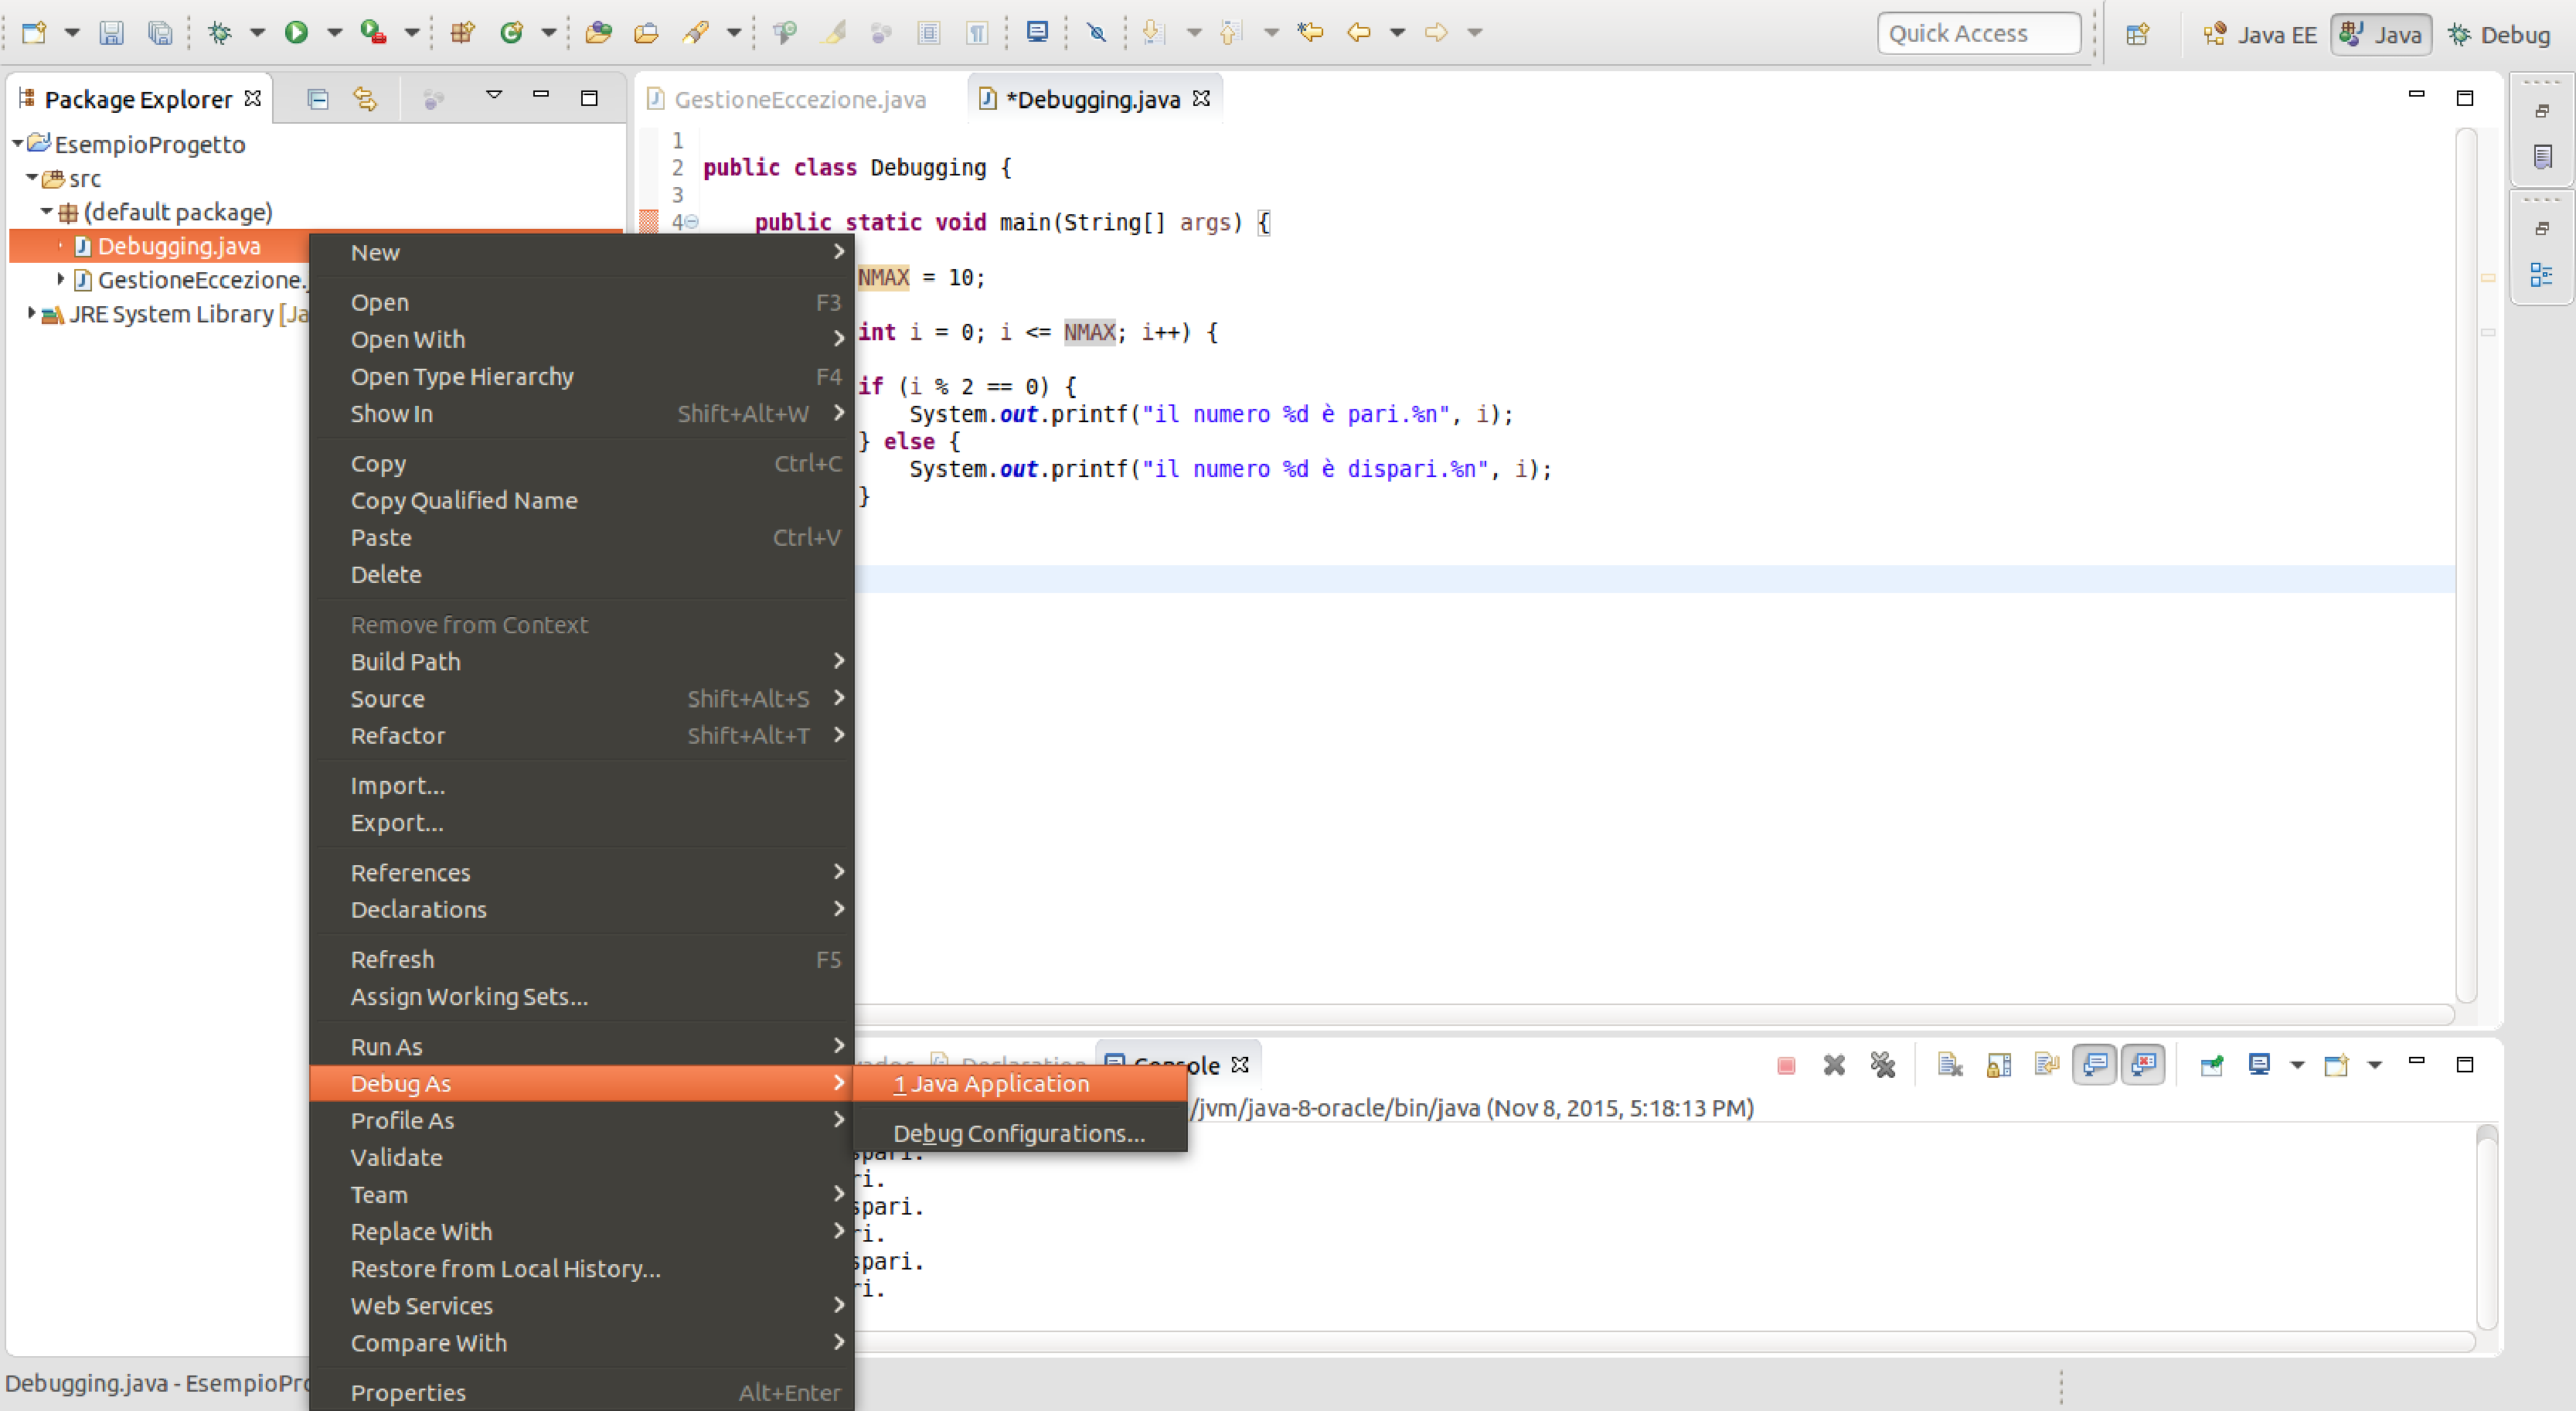
\includepdf[pages={1}]{img/debug/debug01.pdf}
}

\pgfdeclareimage[width=0.5\paperwidth]{debug_perspective}{img/debug/debug_perspective.png}
\begin{frame}{Debugging (V)}

  Confermare l'apertura della \emph{debug perspective}:
  \begin{center}
   \pgfuseimage{debug_perspective}
  \end{center}

\end{frame}

% \pgfdeclareimage[width=0.25\paperwidth]{debug01}{img/debug/debug01.png}
{
  \setbeamercolor{background canvas}{bg=}
  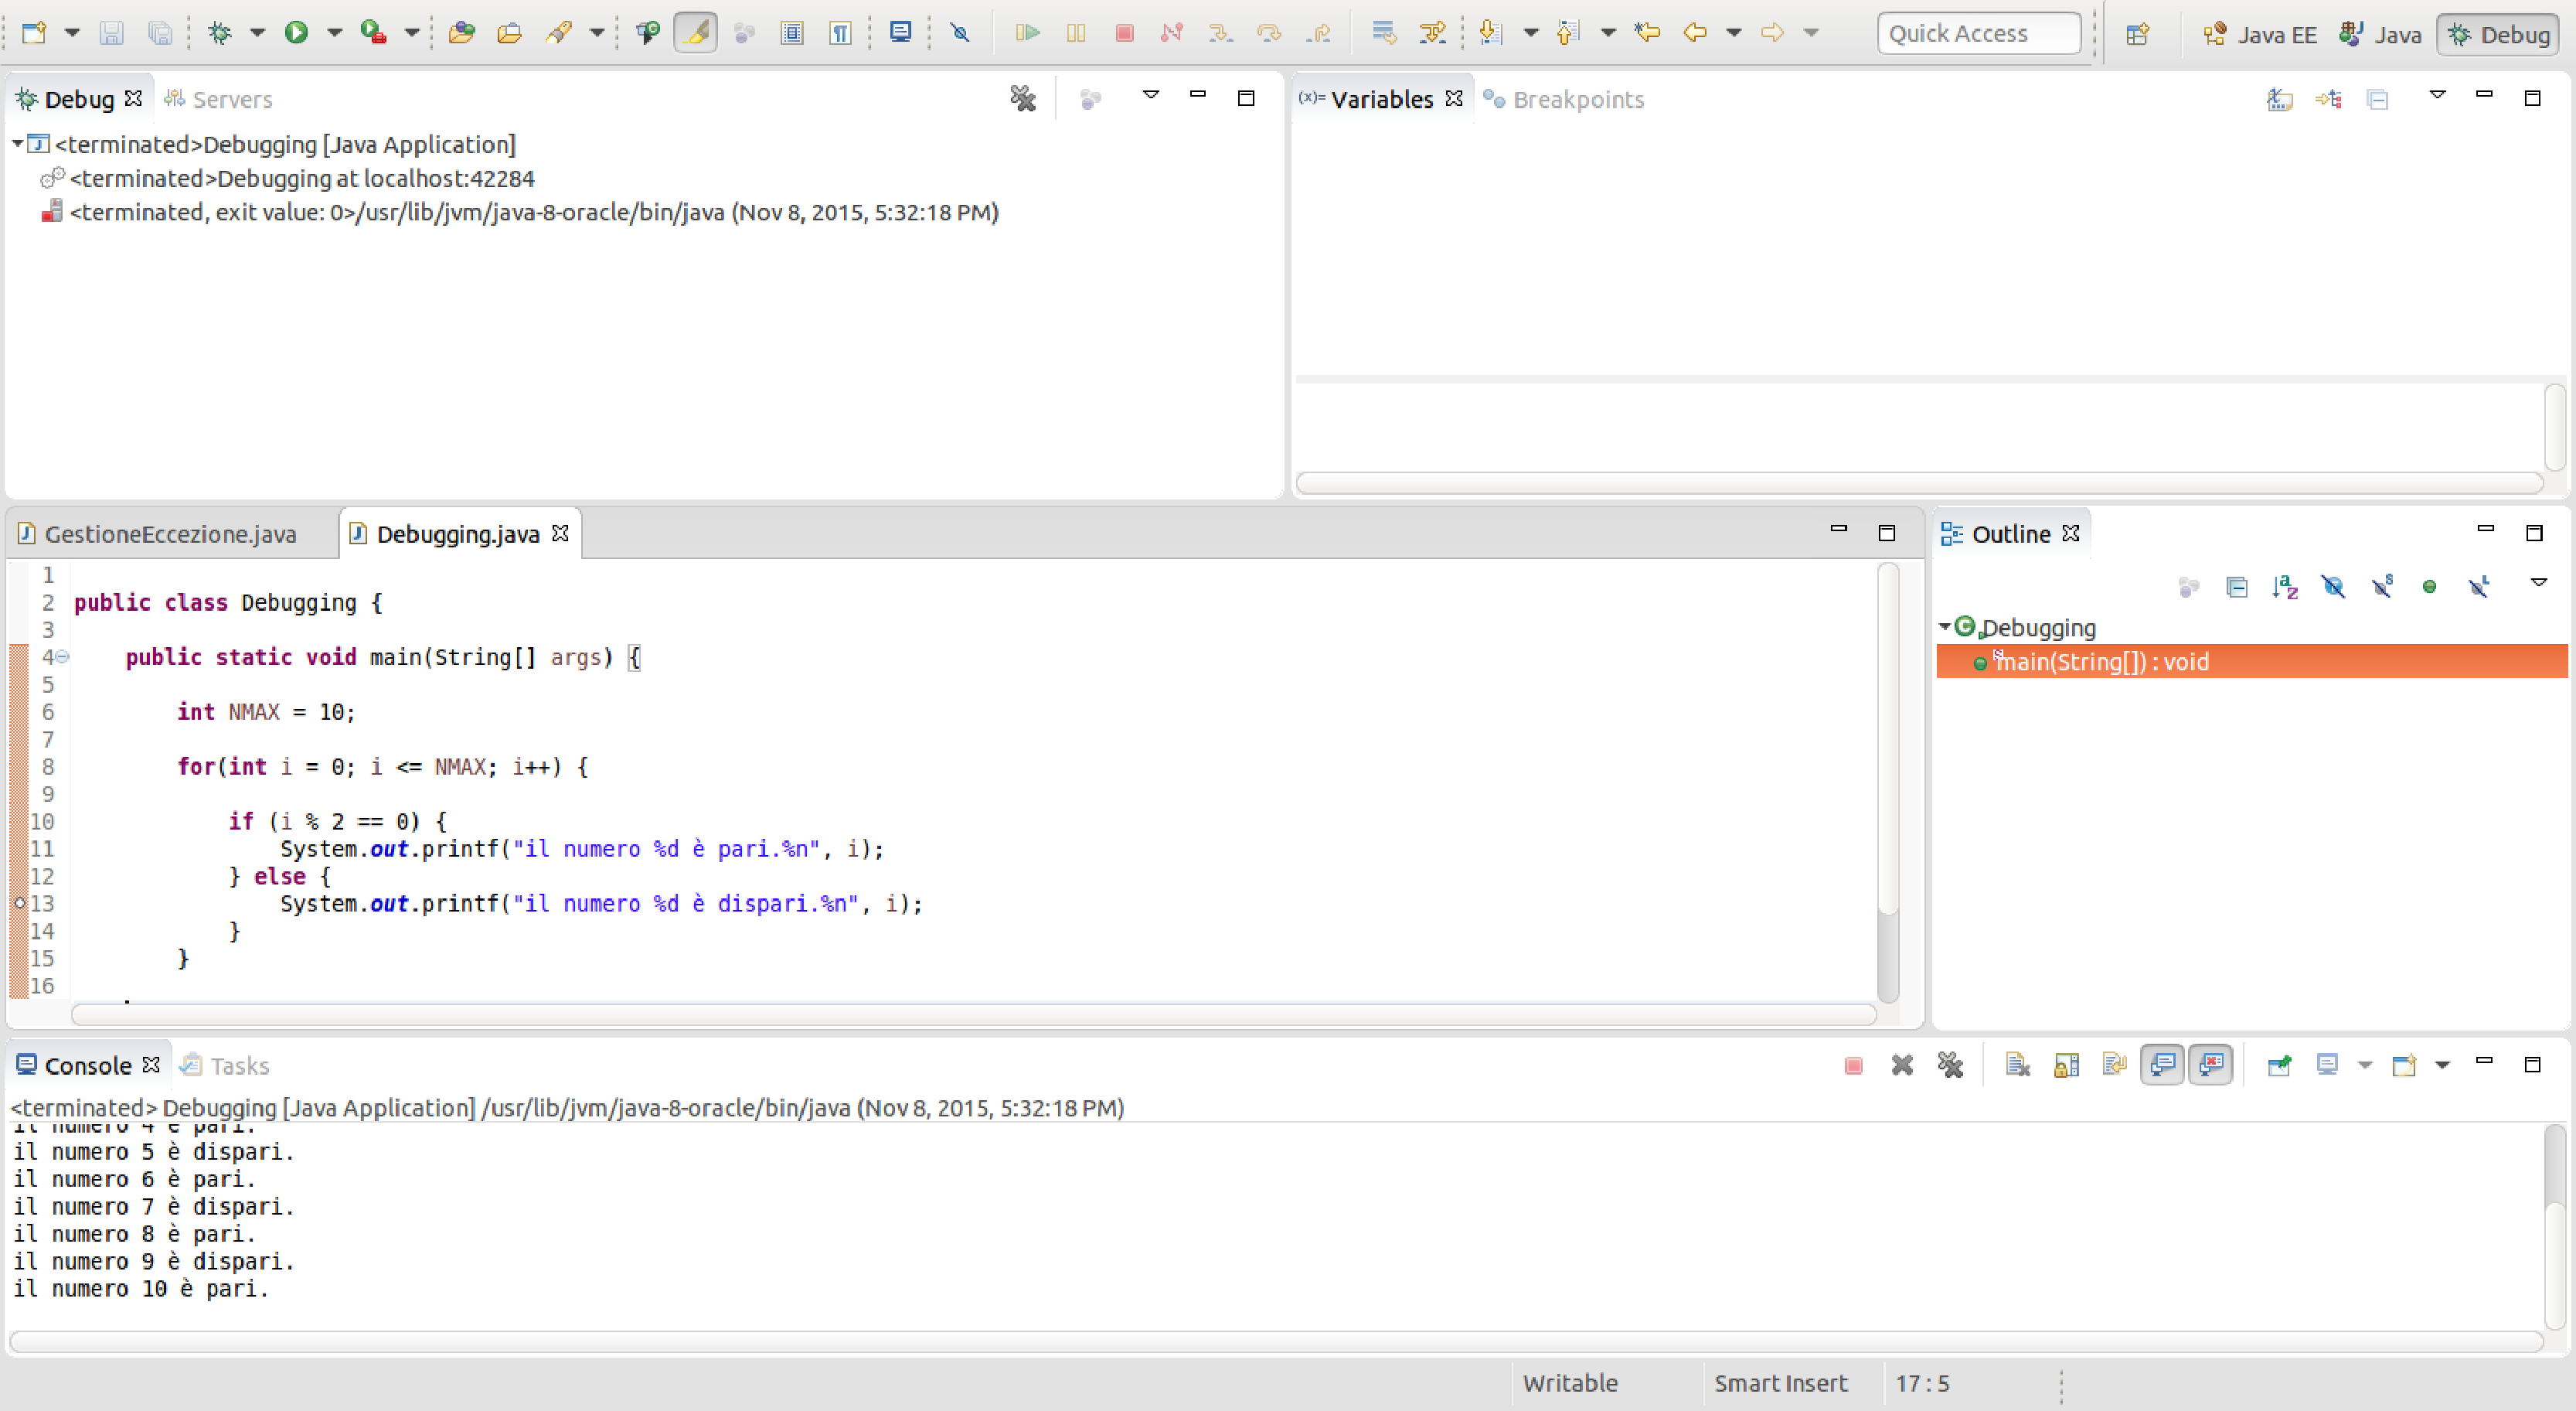
\includepdf[pages={1}]{img/debug/debug02.pdf}
}

{
  \setbeamercolor{background canvas}{bg=}
  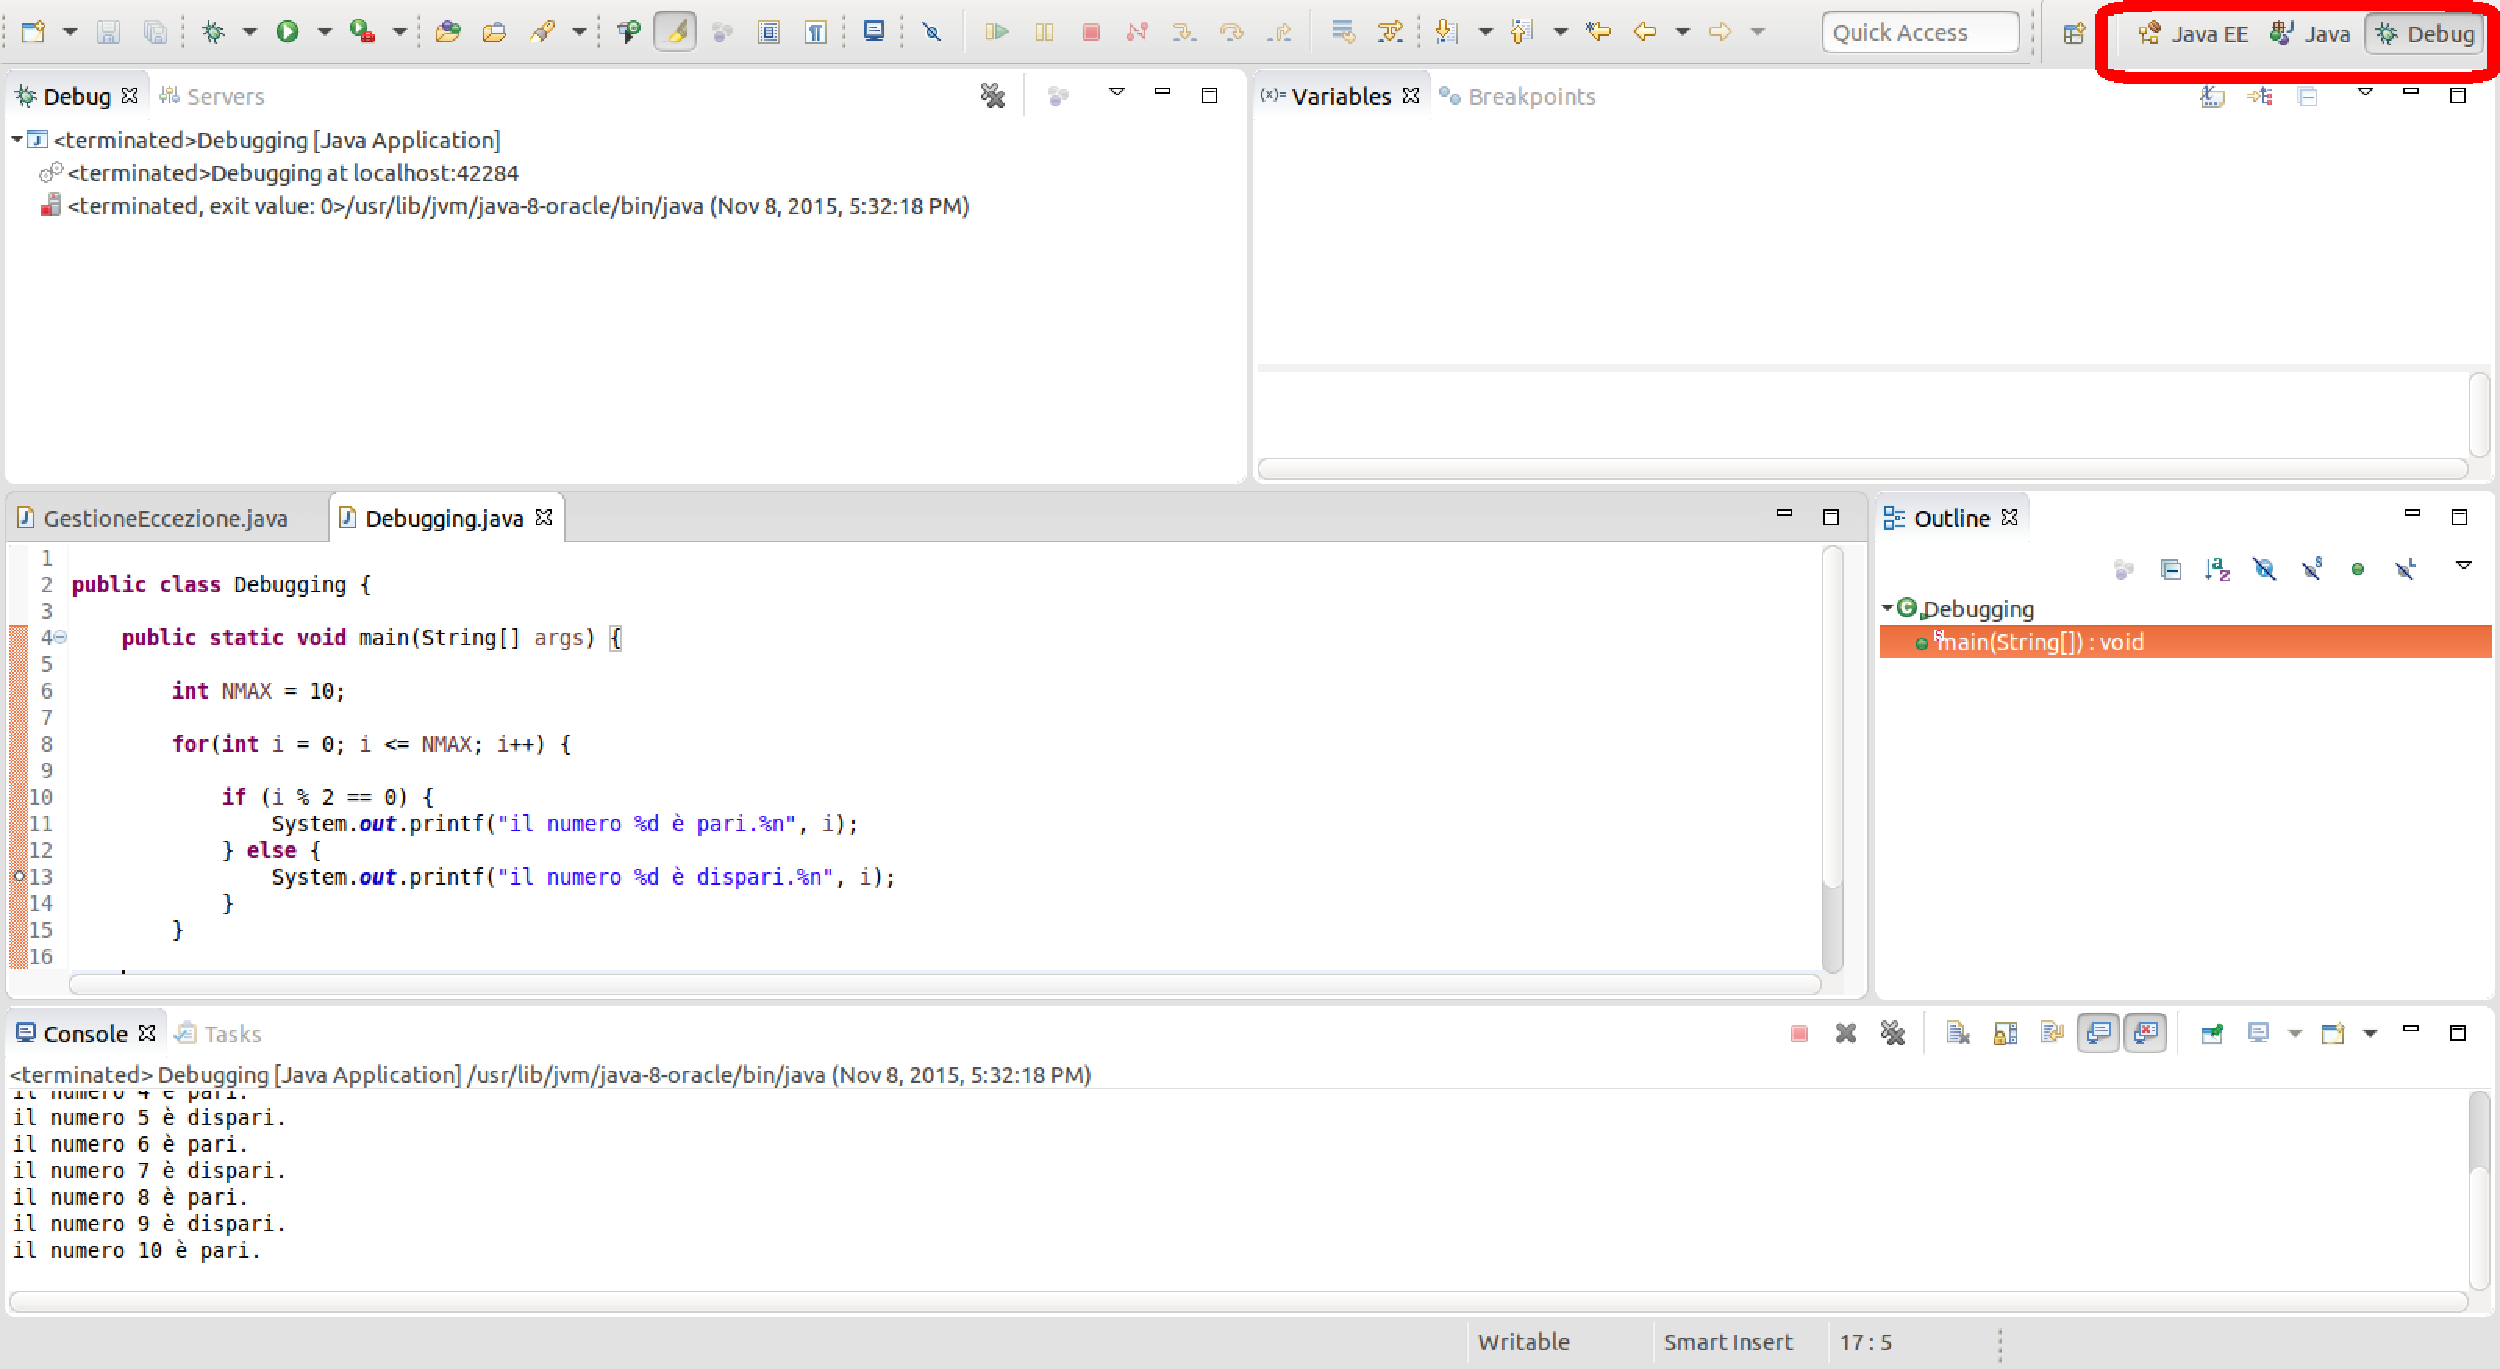
\includepdf[pages={1}]{img/debug/debug03.pdf}
}

{
  \setbeamercolor{background canvas}{bg=}
  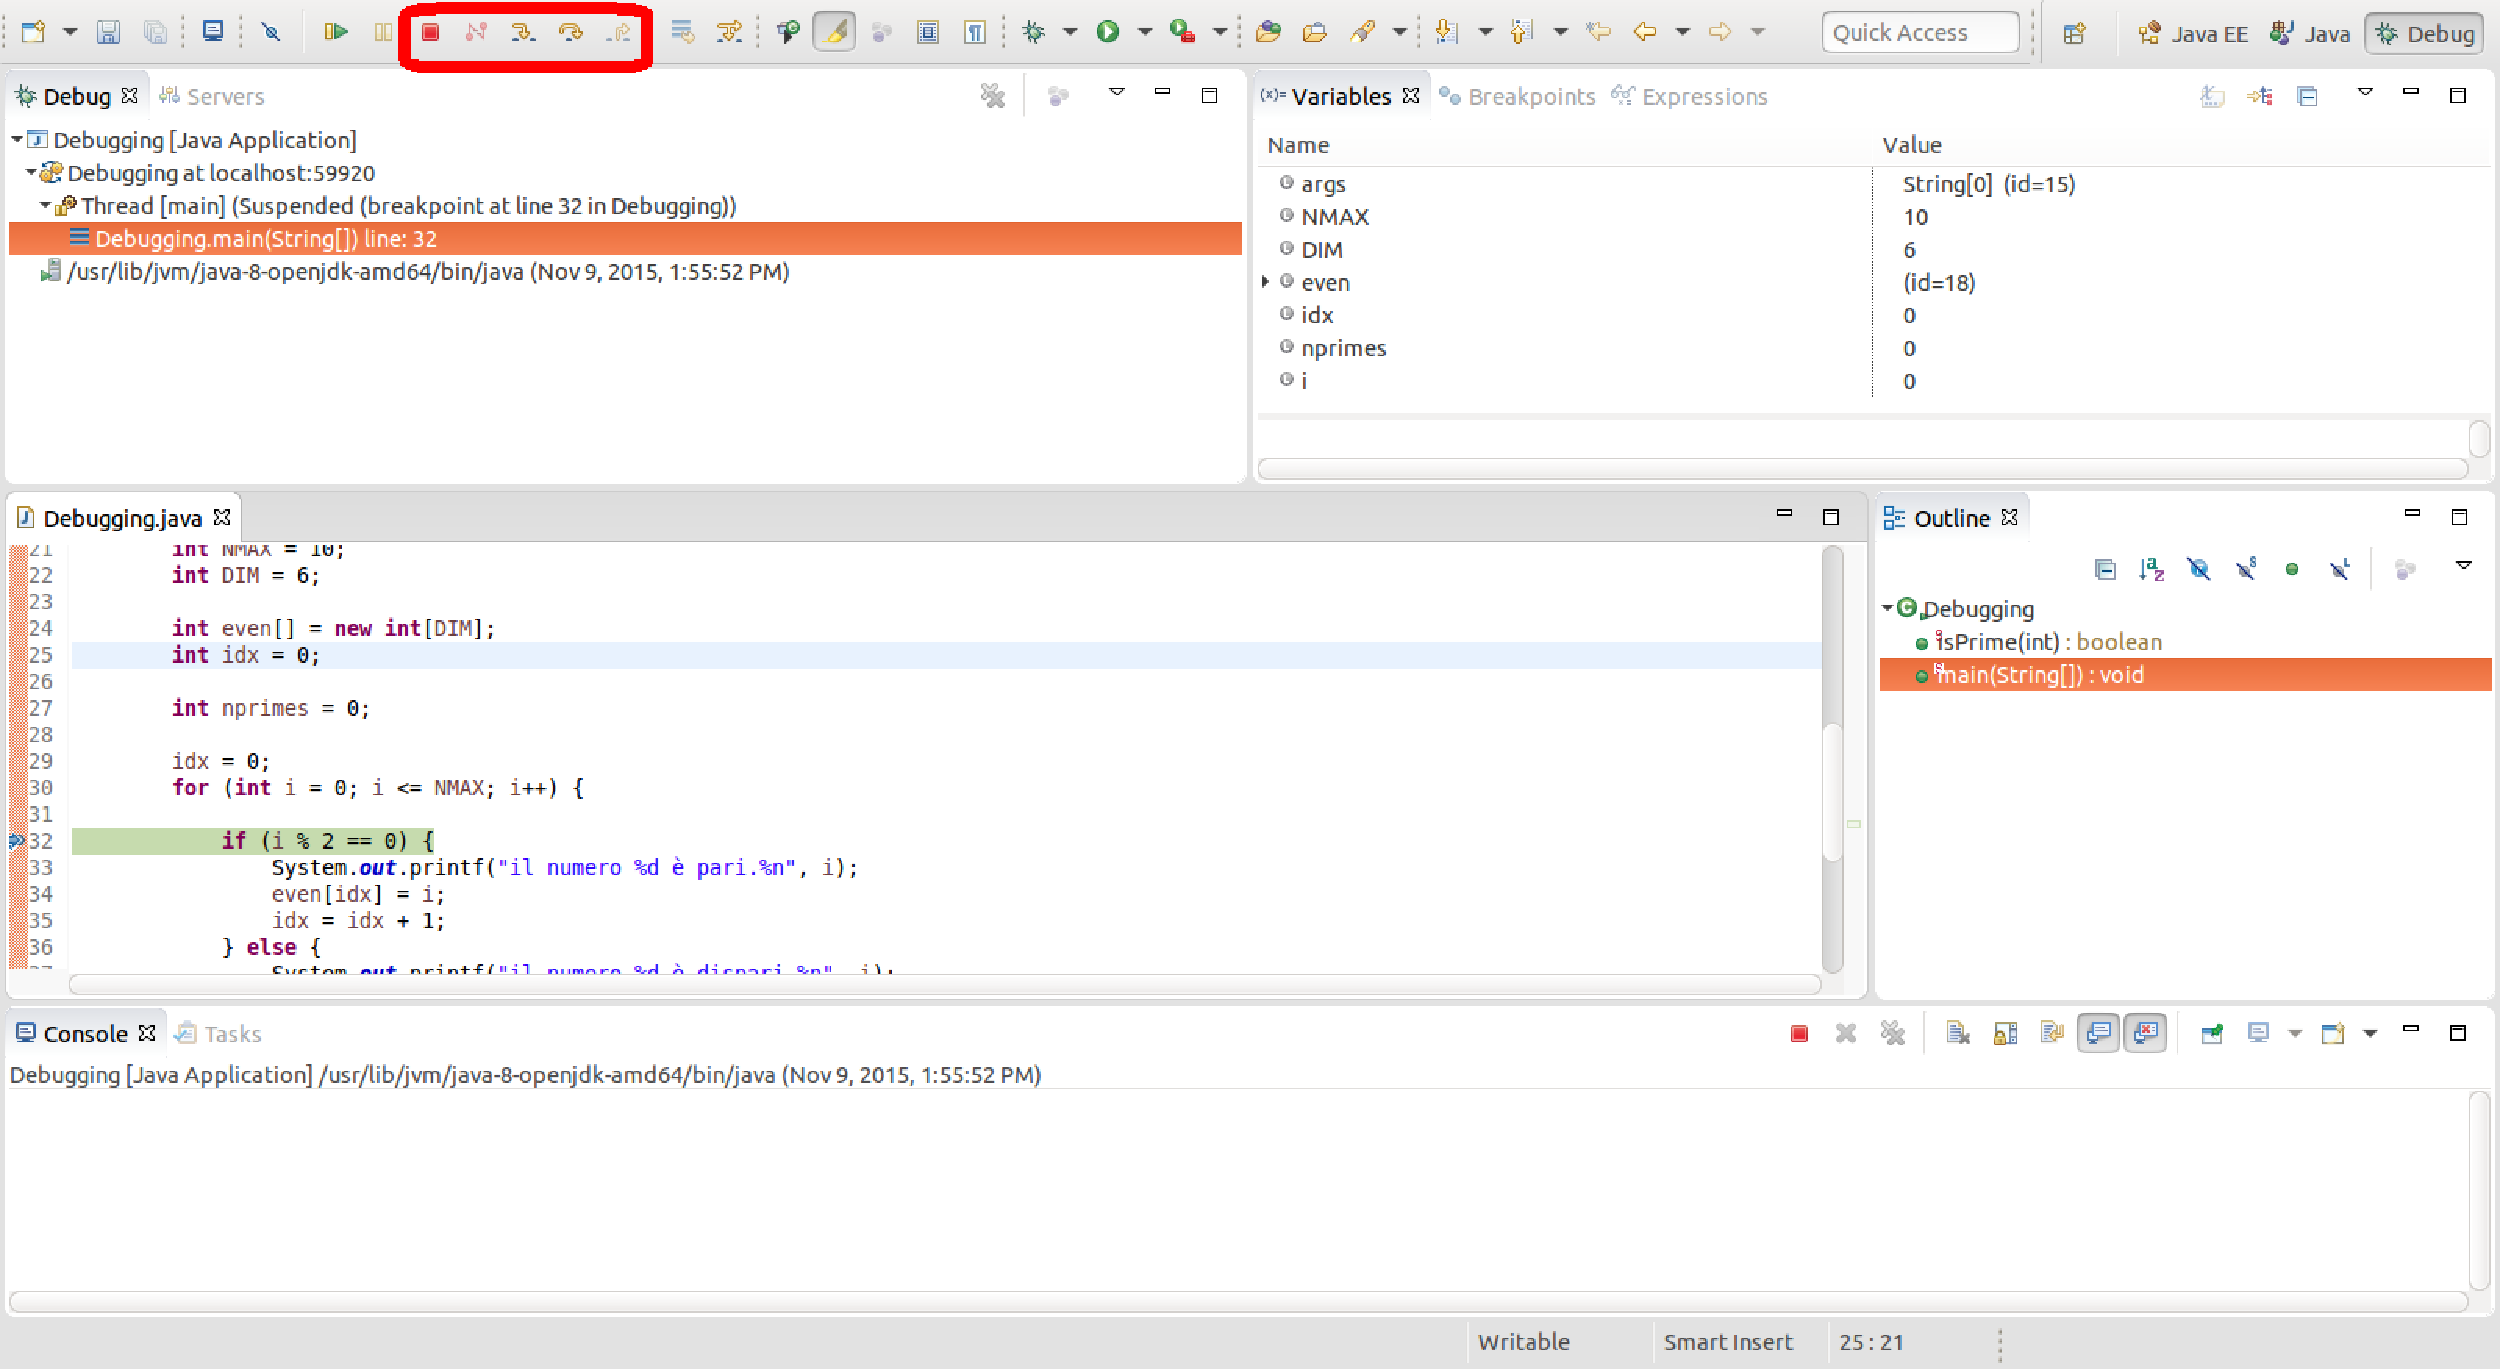
\includepdf[pages={1}]{img/debug/debug04.pdf}
}

\begin{frame}{Debugging (IV)}

  Il debugger pu\`o essere comandato attraverso le icone nella barra o i tasti funzione:
  \begin{itemize}
    \item \textbf{F5} esegue la linea selezionata e va alla riga successiva. Se la linea selezionata \`e una chiamata a funzione allora il debugger entra nella funzione indicata;
    \item \textbf{F6} ``step over'': esegue un metodo senza entrare esplicitamente in esso con il debugger;
    \item \textbf{F7} ``step out'': ritorna alla funzione che ha chiamato il metodo corrent, ovvero termina l'esecuzione del metodo corrente e ritorna al chiamante;
    \item \textbf{F8} riprende l'esecuzione del programma fino a che non viene incontrato un nuovo breakpoint;
  \end{itemize}

\end{frame}

\pgfdeclareimage{debug_buttons02}{img/debug/debug_buttons02.png}
\begin{frame}{Debugging (V)}

  \begin{center}
    \pgfuseimage{debug_buttons02}
  \end{center}

\end{frame}

\begin{frame}{Debugging (VI)}

  Dal pannello \textbf{variabili} è possibile:
  \begin{itemize}
    \item ispezionare il valore della variabile;
    \item (click destro) impostare un nuovo valore per la variabile;
  \end{itemize}

\end{frame}

\pgfdeclareimage{debug_perspective_exit}{img/debug/debug_perspective_exit.png}
\begin{frame}{Debugging (VII)}

  Per uscira dal debugging, ovvero cambiare prospettiva e ritornare alla finestra ``standard''
  di Eclipse, si possono usare i pulsanti posti in altro a destra:

  \begin{center}
    \pgfuseimage{debug_perspective_exit}
  \end{center}
\end{frame}


\section{Esercizi}
\subsection[Esercizi]{Esercizi}

\begin{frame}{Esercizi (I)}
  \begin{itemize}
   \item Scrivete un programma che stampi la canzone popolare inglese ``\emph{99 bottiglie di birra}''
   \item (vedete anche \url{https://esolangs.org/wiki/99_bottles_of_beer})
  \end{itemize}
  \begin{quote}
   «99 bottles of beer on the wall, 99 bottles of beer.\newline
   Take one down, pass it around, 98 bottles of beer on the wall \newline
   99 bottles of beer on the wall, 99 bottles of beer.\newline
   Take one down, pass it around, 98 bottles of beer on the wall  \newline
   ...\newline
   1 bottle of beer on the wall, 1 bottle of beer.\newline
   Take one down, pass it around, no more bottles of beer on the wall\newline
   There no more bottles of beer on the wall, no more bottles of beer.»
  \end{quote}

\end{frame}

\begin{frame}{Esercizi (II)}
  \begin{itemize}
    \item Utilizzando il ciclo \texttt{while} scrivete un programma che dato un 
    intero stampi a schermo la ``tabellina''.
    Ad esempio, se il numero è 7 dovrete stampare a schermo:
    \begin{itemize}
      \item 7*0 = 0
      \item 7*1 = 7
      \item 7*2 = 14
      \item $\dots$
      \item 7*10 = 70
    \end{itemize}
    \item riscrivete il programma precendente usando il ciclo \texttt{for}.
  \end{itemize}
\end{frame}


\begin{frame}{Esercizi (III)}
  \begin{itemize}
   \item Scrivete un programma che calcoli il fattoriale di un numero intero a vostra scelta.
  \end{itemize}

  La definizione del fattoriale è la seguente:
  \begin{equation}
    n! = n \times (n - 1) \times \dots \times 1
  \end{equation}
  quindi il calcolo del fattoriale può essere definito da: 
  \begin{center}
    \begin{minipage}{8cm}
      \begin{algorithmic}[1]
	\State $fatt \gets ?$ \Comment Quale valore va messo qui?
	\For{$i \gets 1$ to $N$}
	  \State $fatt \gets fatt \times i$ 
	\EndFor
      \end{algorithmic}
   \end{minipage}
  \end{center}

\end{frame}

\begin{frame}{Esercizi (IV)}
  \begin{itemize}
    \item Scrivere un programma che stampi i valori della serie di Fibonacci minori di 10000.
    La serie di Fibonacci \`e definita da:
    \begin{equation*}
      \left\{\begin{aligned}
	  & x_0 = 1\\
	  & x_1 = 1\\
	  & x_{n+1} = x_{n} + x_{n-1}
      \end{aligned}\right.
    \end{equation*}
  \end{itemize}

\end{frame}


\begin{frame}{Esercizi (V)}
  \begin{itemize}
    \item Scrivere un programma che usi il metodo per il calcolo della radice quadrata di Newton.
    
    \begin{equation*}
      \left\{\begin{aligned}
	  & x_0 = 0.5\\
	  & x_{n +1} = 0.5 \cdot {x_n} (3  - zx^2_n)
      \end{aligned}\right.
    \end{equation*}
    \begin{equation*}
     \lim_{n \to \infty} x_{n} = \sqrt{z}
    \end{equation*}
  \end{itemize}
  
  Il programma deve calcolare la serie definita sopra fino a che l'errore $\varepsilon_{n} = |x^{2}_{n} - z|$,
  non è più piccolo di $10^{-3}$. Per il valore assoluto utilizzate la funzione \texttt{Math.\Blue{abs()}}.

\end{frame}

\begin{frame}{Esercizi (VI)}
  \begin{itemize}
    \item Metodo della bisezione
  \end{itemize}
  \begin{tiny}
    \url{https://ece.uwaterloo.ca/~dwharder/NumericalAnalysis/10RootFinding/bisection/bisection.gif}
  \end{tiny}

  \begin{scriptsize}
    \begin{center}
      \begin{minipage}{8cm}
	\begin{algorithmic}[1]
	  \Require Function $f$, endpoint values $a, b$, tolerance $\varepsilon$, maximum iterations $N_{MAX}$
		   $a < b$, either $f(a) < 0$ and $f(b) > 0$ or $f(a) > 0$ and $f(b) < 0$
	  \Ensure value which differs from $a$ root of $f(x)=0$ by less than $\varepsilon$
    
	  \State $N \gets 1$
	  \While{$N \leq N_{MAX}$}
	    \State $c \gets (a + b)/2$
	    \If{$f(c) = 0 \lor (b – a)/2 < \varepsilon$}
	      \State \texttt{\textbf{print}}(c)
	      \State \Return;
	    \EndIf
	    \State $N \gets N + 1$
	    \If{$sign(f(c)) = sign(f(a))$}
	      \State $a \gets c$
	    \Else 
	      \State $b \gets c$
	    \EndIf
	  \EndWhile
	  \State \texttt{\textbf{print}}(Non ho trovato risultati)
	\end{algorithmic}
      \end{minipage}
    \end{center}
  \end{scriptsize}

\end{frame}

\begin{frame}{Esercizi (VII)}
  Test di primalità
  \begin{itemize}
    \item Scrivere un programma che, dato un intero positivo, verifichi se quel numero è primo oppure no.
  \end{itemize}

   Un numero $n \in \mathbb{N}, n > 1$ \`e \textbf{primo} se e solo se \`e divisibile solo per $1$ e per
   se stesso.
\end{frame}

% \appendix
% \section*{Backup}
% \begin{frame}
\begin{Huge}
Backup 
\end{Huge}
\end{frame}


\end{document}
